\documentclass[12pt]{article}
\usepackage[margin=0.75in]{geometry}
\usepackage{float}
\usepackage{multicol}
\usepackage{lmodern}
\usepackage{amssymb,amsmath}
\usepackage{ifxetex,ifluatex}
\usepackage{fixltx2e} % provides \textsubscript
\ifnum 0\ifxetex 1\fi\ifluatex 1\fi=0 % if pdftex
  \usepackage[T1]{fontenc}
  \usepackage[utf8]{inputenc}
\else % if luatex or xelatex
  \ifxetex
    \usepackage{mathspec}
    \usepackage{xltxtra,xunicode}
  \else
    \usepackage{fontspec}
  \fi
  \defaultfontfeatures{Mapping=tex-text,Scale=MatchLowercase}
  \newcommand{\euro}{€}
\fi
% use upquote if available, for straight quotes in verbatim environments
\IfFileExists{upquote.sty}{\usepackage{upquote}}{}
% use microtype if available
\IfFileExists{microtype.sty}{%
\usepackage{microtype}
\UseMicrotypeSet[protrusion]{basicmath} % disable protrusion for tt fonts
}{}
\usepackage{longtable,booktabs}
\usepackage{graphicx}
\makeatletter
\def\maxwidth{\ifdim\Gin@nat@width>\linewidth\linewidth\else\Gin@nat@width\fi}
\def\maxheight{\ifdim\Gin@nat@height>\textheight\textheight\else\Gin@nat@height\fi}
\makeatother
% Scale images if necessary, so that they will not overflow the page
% margins by default, and it is still possible to overwrite the defaults
% using explicit options in \includegraphics[width=3.5in][width, height, ...]{}
\setkeys{Gin}{width=\maxwidth,height=\maxheight,keepaspectratio}
\ifxetex
  \usepackage[setpagesize=false, % page size defined by xetex
              unicode=false, % unicode breaks when used with xetex
              xetex]{hyperref}
\else
  \usepackage[unicode=true]{hyperref}
\fi
\hypersetup{breaklinks=true,
            bookmarks=true,
            pdfauthor={Brandon LeBeau},
            pdftitle={PSQF 4143: Section 10},
            colorlinks=true,
            citecolor=blue,
            urlcolor=blue,
            linkcolor=magenta,
            pdfborder={0 0 0}}
\urlstyle{same}  % don't use monospace font for urls
\setlength{\parindent}{0pt}
\setlength{\parskip}{6pt plus 2pt minus 1pt}
\setlength{\emergencystretch}{3em}  % prevent overfull lines
\setcounter{secnumdepth}{0}

\title{PSQF 4143: Section 10}
\author{Brandon LeBeau}
\date{}

\begin{document}
\maketitle

\section{Dichotomous Populations}\label{dichotomous-populations}

\begin{figure}[H]
\centering
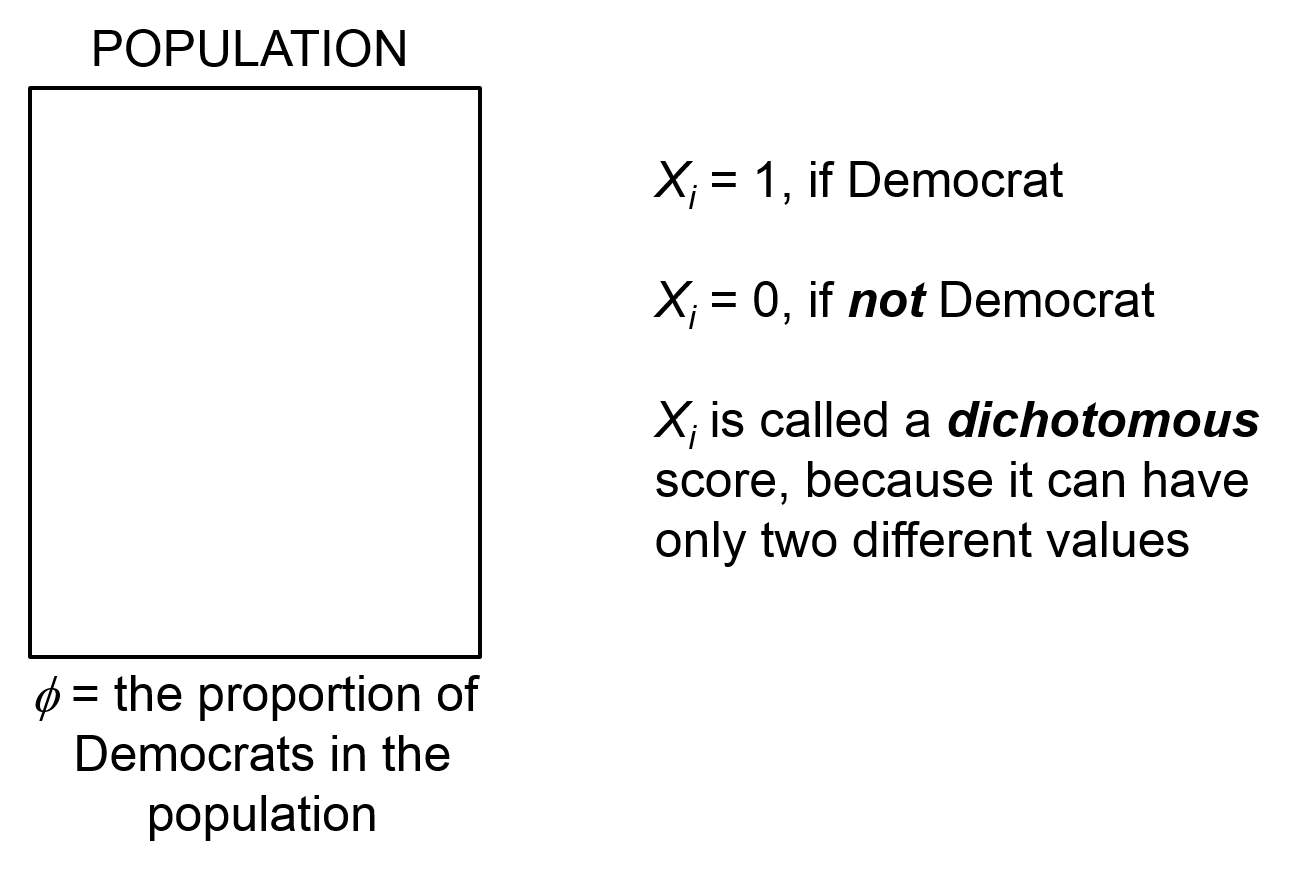
\includegraphics[width=3.5in]{dich_population.png}
\caption{}
\end{figure}

\section{Dichotomous Populations 2}\label{dichotomous-populations-2}

\[ \phi = \frac{\mbox{# of Democrats}}{N} \]
\[ \phi = \frac{\sum X_{i}}{N} \]

\begin{itemize}
\itemsep1pt\parskip0pt\parsep0pt
\item
  Thus, \(\phi\) is the mean of the population of dichotomous scores
\item
  More simply, \(\phi = \mu\)
\end{itemize}

\section{Dichotomous Populations 3}\label{dichotomous-populations-3}

\begin{itemize}
\itemsep1pt\parskip0pt\parsep0pt
\item
  Recall: \(\sigma^2 = \frac{\sum X_{i}^{2}}{N} - \mu^2\)
\item
  Now: because \(X_{i}\) is dichotomous, \(X_{i}^{2} = X_{i}\)
\item
  Therefore: \[\sigma^{2} = \frac{\sum X_{i}}{N} - \mu^2\]
  \[\sigma^2 = \phi - \phi^2\] \[ \sigma^2 = \phi (1 - \phi)\]
\end{itemize}

\section{The sampling distribution of the
proportion}\label{the-sampling-distribution-of-the-proportion}

\begin{figure}[H]
\centering
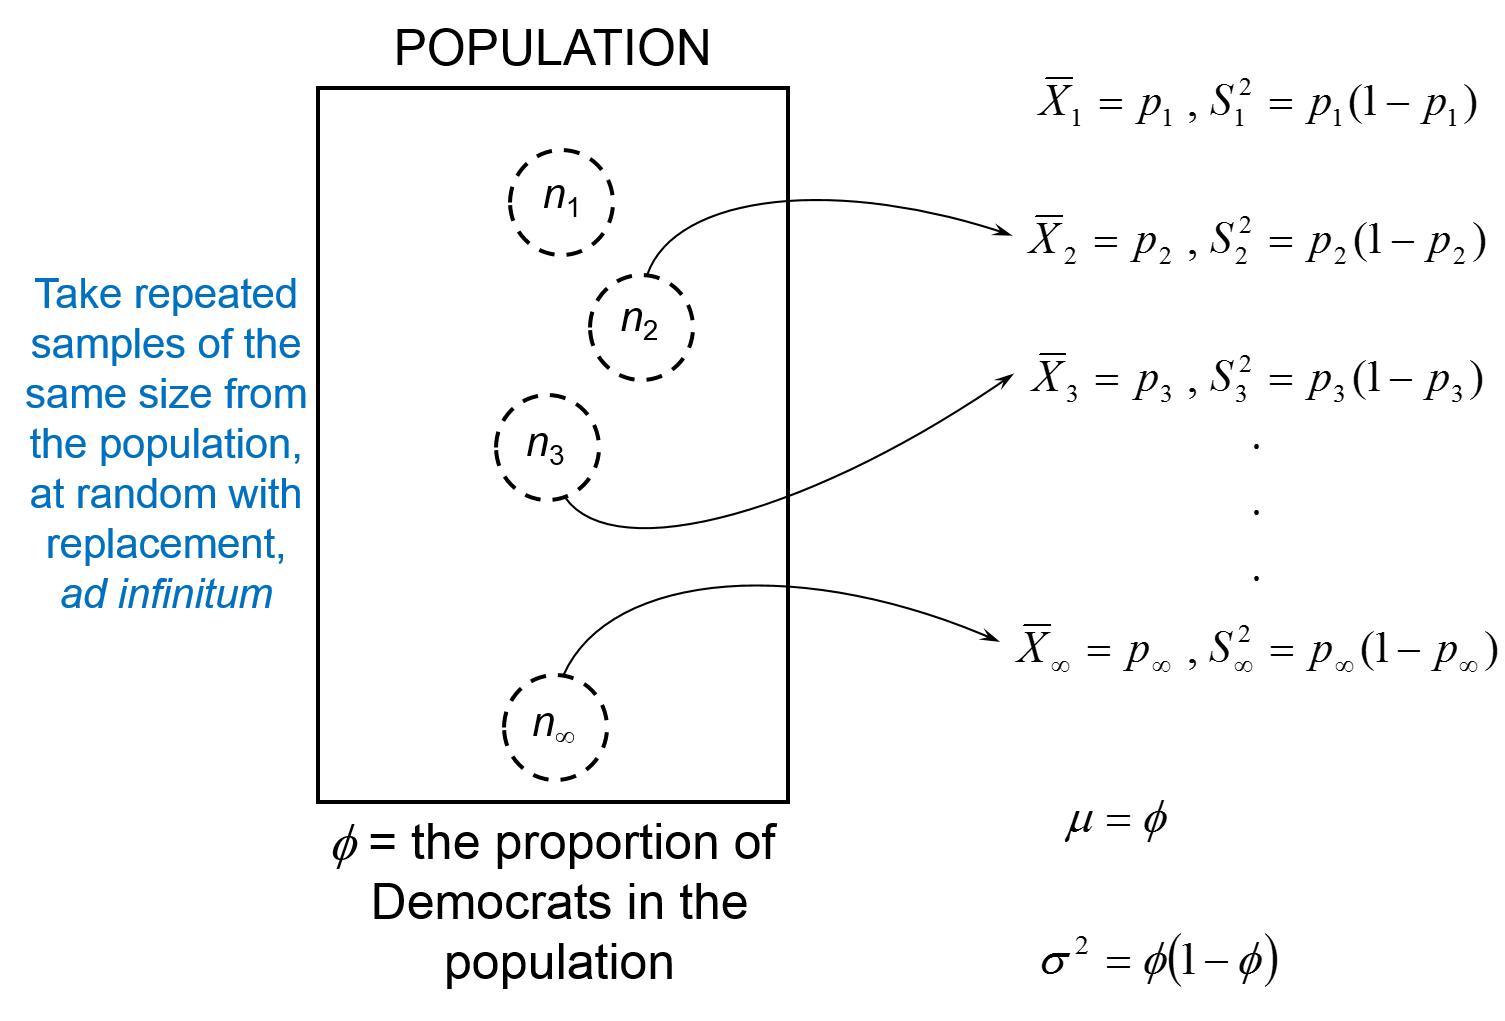
\includegraphics[width=3.5in]{sample_dist_proportion.png}
\caption{}
\end{figure}

\section{The sampling distribution of the proportion
2}\label{the-sampling-distribution-of-the-proportion-2}

\begin{itemize}
\itemsep1pt\parskip0pt\parsep0pt
\item
  Definition:

  \begin{itemize}
  \itemsep1pt\parskip0pt\parsep0pt
  \item
    Given an infinite dichotomous population, the elements of which are
    assigned a score of 1 if they belong to Class A and a score of 0 if
    they do not belong to Class A, the sampling distribution of the
    proportion p in random samples of size n taken from this population,
    approaches the normal distribution with:
  \end{itemize}
\end{itemize}

\section{Sampling disribution of the proportion
3}\label{sampling-disribution-of-the-proportion-3}

\begin{itemize}
\itemsep1pt\parskip0pt\parsep0pt
\item
  Mean: \(\mu_{p} = \phi\)
\item
  Variance: \(\sigma_{p}^{2} = \frac{\phi (1 - \phi)}{n}\)
\item
  SD: \(\sigma_{p} = \sqrt{\frac{\phi (1 - \phi)}{n}}\)
\end{itemize}

as \(n\) increases: - Variance:
\(\sigma_{\bar{X}}^{2} = \frac{\sigma_{X}^2}{n}\) - SD:
\(\sigma_{\bar{X}} = \frac{\sigma_{X}}{\sqrt{n}}\)

\begin{itemize}
\itemsep1pt\parskip0pt\parsep0pt
\item
  Note:

  \begin{itemize}
  \itemsep1pt\parskip0pt\parsep0pt
  \item
    This approximation (to the normal distribution) improves as \(n\)
    gets larger, and the closer \(\phi\) is to 0.5.
  \item
    The farther away \(\phi\) is away from 0.5, and the smaller \(n\),
    the worse the approximation to the normal distribution.
  \end{itemize}
\end{itemize}

\section{Normal Approximation Example (n = 5; p =
0.5)}\label{normal-approximation-example-n-5-p-0.5}

\begin{figure}[H]
\centering
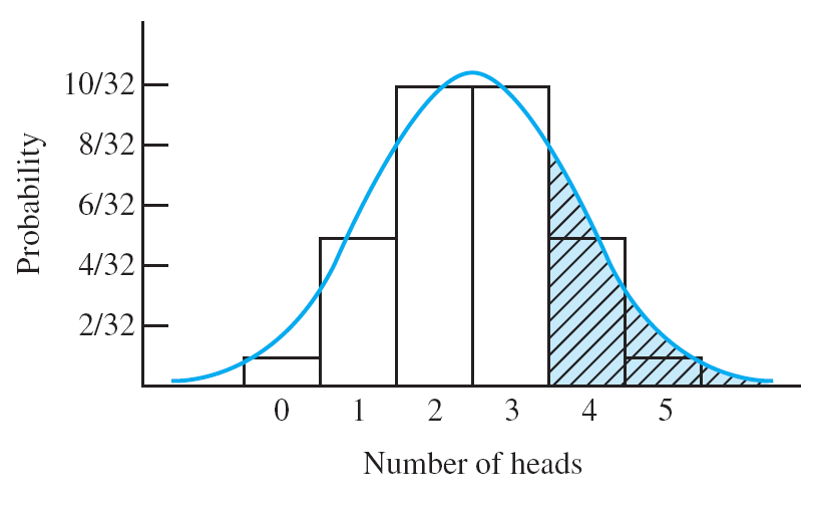
\includegraphics[width=3.5in]{binom_norm_approx.png}
\caption{}
\end{figure}

\begin{itemize}
\itemsep1pt\parskip0pt\parsep0pt
\item
  These probabilities can be looked up from the binomial table in the
  course packet.
\end{itemize}

\section{Sampling distribution of the proportion
4}\label{sampling-distribution-of-the-proportion-4}

\begin{itemize}
\itemsep1pt\parskip0pt\parsep0pt
\item
  The sampling distribution of the proportion follows the binomial
  distribution
\item
  It is known that the normal distribution provides a good approximation
  to the binomial distribution when n is large
\item
  Here, we have chosen the normal distribution as an approximation to
  the sampling distribution of proportion, rather than using its true
  binomial sampling distribution
\end{itemize}

\section{Sampling distribution of the proportion
5}\label{sampling-distribution-of-the-proportion-5}

\begin{itemize}
\itemsep1pt\parskip0pt\parsep0pt
\item
  There are three reasons for doing this:

  \begin{enumerate}
  \def\labelenumi{\arabic{enumi}.}
  \itemsep1pt\parskip0pt\parsep0pt
  \item
    \(p\) is a special case of \(\bar{X} | X_{i} = {0 \mbox{ or } 1}\)

    \begin{itemize}
    \itemsep1pt\parskip0pt\parsep0pt
    \item
      As such, a sampling theory for \(p\) is easily derived from a
      sampling theory for the mean.
    \end{itemize}
  \item
    The normal distribution is a commonly used probability model.
  \item
    Based on the assumption of large samples.
  \end{enumerate}
\end{itemize}

\section{Example 1}\label{example-1}

\begin{itemize}
\itemsep1pt\parskip0pt\parsep0pt
\item
  A few days before the 2008 presidential election, an ABC
  News/Washington Post tracking poll surveyed a national random sample
  of 2,172 likely voters including landline and cell-phone-only
  respondents
\item
  1,173 of those surveyed said they would vote for Barack Obama -Conduct
  a hypothesis test at the a = .05 level of significance to determine
  whether a majority of the population of likely voters would vote for
  Barack Obama
\end{itemize}

\section{Example 2}\label{example-2}

\begin{itemize}
\itemsep1pt\parskip0pt\parsep0pt
\item
  A news reporter wants to investigate the advertising claim that a
  particular speed reading course will ``help to improve reading
  comprehension''
\item
  She decides to conduct the following experiment:

  \begin{enumerate}
  \def\labelenumi{\arabic{enumi}.}
  \itemsep1pt\parskip0pt\parsep0pt
  \item
    Select 200 freshman at random from all UI freshman. What is the EAP?
    What is the TP?
  \item
    Form 100 matched pairs (using ACT Reading scores).
  \item
    Randomly assign one member of each pair to the speed reading course
    (assume all students will participate).
  \item
    After the course is completed, administer a reading achievement test
    to all 200 students.
  \item
    For each pair of students, subtract the reading score of the control
    student from that of the experimental student.
  \item
    For these 100 difference scores, calculate the proportion (p) that
    are positive (greater than 0). This proportion is the outcome
    (statistic) of interest.
  \end{enumerate}
\end{itemize}

\section{Example 2 continued}\label{example-2-continued}

\begin{itemize}
\itemsep1pt\parskip0pt\parsep0pt
\item
  After completing the experiment, the news reporter found that 65\% (p
  = 0.65) of the difference scores were positive
\item
  Conduct a hypothesis test at the \(\alpha = .10\) level of
  significance to determine whether the speed reading course was
  effective in increasing reading comprehension in the population of UI
  freshman

  \begin{itemize}
  \itemsep1pt\parskip0pt\parsep0pt
  \item
    What is the interpretation of \(\alpha = .10\)?
  \end{itemize}
\end{itemize}

\section{Calculating a confidence
interval}\label{calculating-a-confidence-interval}

\begin{itemize}
\itemsep1pt\parskip0pt\parsep0pt
\item
  Suppose we wanted to calculate a 95\% confidence interval for \(\phi\)
  of the 2008 presidential election data.

  \begin{itemize}
  \itemsep1pt\parskip0pt\parsep0pt
  \item
    \(n = 2172, p = 0.54\)
  \end{itemize}
\end{itemize}

\section{Calculating a confidence interval -
specifics}\label{calculating-a-confidence-interval---specifics}

\[ \hat{\sigma}_{p} = \sqrt{\frac{p (1 - p)}{n - 1}} \]
\[ CI = p \pm z_{crit} * \hat{\sigma}_{p} \] where \(z_{crit}\) is based
on the level of confidence or \(1 - \alpha\).

\section{Interpretting a confidence
interval}\label{interpretting-a-confidence-interval}

\begin{itemize}
\itemsep1pt\parskip0pt\parsep0pt
\item
  How is the confidence interval: \(c(0.52 \leq \phi \leq 0.56) = .95\)
  interpretted?

  \begin{itemize}
  \itemsep1pt\parskip0pt\parsep0pt
  \item
    Does \(\phi\) fall in the interval?
  \item
    Is there a 95\% chance that \(\phi\) falls in this interval?
  \item
    Do we know if \(\phi\) falls in the interval?
  \item
    If we construct 100 such intervals, how many would contain \(\phi\)?
  \item
    If we were to construct an infinite number of intervals, how many
    would contain \(\phi\)?
  \end{itemize}
\end{itemize}

\section{Using Confidence interval to do hypothesis
testing}\label{using-confidence-interval-to-do-hypothesis-testing}

\begin{itemize}
\itemsep1pt\parskip0pt\parsep0pt
\item
  You can use a 95\% confidence interval to conduct a two-tailed test of
  any null hypothesis at the specificied \(\alpha\) level.
\item
  If the hypothesized value falls within the confidence interval, fail
  to reject \(H_{0}\) (retain \(H_{0}\)).
\item
  If the hypothesized value falls outside the confidence interval,
  reject \(H_{0}\).
\item
  Example:

  \begin{itemize}
  \itemsep1pt\parskip0pt\parsep0pt
  \item
    \(H_{0}: \phi = 0.5\)
  \item
    \(H_{1}: \phi \neq 0.5\)
  \item
    \(c(0.52 \leq \phi \leq 0.56) = .95\), \(\alpha = 0.05\)
  \item
    0.5 lies outside of 95\% confidence interval, therefore, reject
    \(H_{0}\)
  \end{itemize}
\end{itemize}

\section{Summary of one-sample hypothesis
tests}\label{summary-of-one-sample-hypothesis-tests}

\begin{longtable}[c]{@{}lrrr@{}}
\toprule
\(H_{0}\) & Standard Error & Test Statistic & Confidence
Interval\tabularnewline
\midrule
\endhead
\(\mu = constant\); \(\sigma_{x}\) known &
\(\sigma_{\bar{X}} = \frac{\sigma_{X}}{\sqrt{n}}\) &
\(z = \frac{\bar{X} - \mu_{0}}{\sigma_{\bar{X}}}\) &
\(\bar{X} \pm \sigma_{\bar{X}} * z_{crit}\)\tabularnewline
\(\mu = constant\); \(\sigma_{x}\) unknown &
\(\hat{\sigma}_{\bar{X}} = \frac{s_{X}}{\sqrt{n - 1}}\); \(df = n - 1\)
& \(t_{n - 1} = \frac{\bar{X} - \mu_{0}}{\hat{\sigma}_{\bar{X}}}\) &
\(\bar{X} \pm \hat{\sigma}_{\bar{X}} * t_{crit(n - 1)}\)\tabularnewline
\(\phi = constant\) &
\(\sigma_{p} = \sqrt{\frac{\phi_{0} (1 - \phi_{0})}{n}}\) &
\(z = \frac{p - \phi_{0}}{\sigma_{p}}\) &
\(p \pm \hat{\sigma}_{p} * z_{crit}\);
\(\hat{\sigma}_{p} = \sqrt{\frac{p (1 - p)}{n - 1}}\)\tabularnewline
\bottomrule
\end{longtable}

\end{document}
